\documentclass[aspectratio=169,slidestop,mathserif]{beamer}

\usepackage{systeme, mathtools}
\usepackage[UTF8,scheme=plain]{ctex}
%\usepackage{pgf}
%\usepackage{listings}
\usepackage{ulem}
\usepackage{color}
\usepackage{graphics,graphicx}
\usepackage{tikz,pgfkeys}
\usepackage{tkz-graph}
\usetikzlibrary{quotes}
\usetikzlibrary{arrows,shapes,shadows, matrix}
\usetikzlibrary{backgrounds,decorations,shapes.misc,positioning,scopes,automata,fit} 
\usetikzlibrary{calc,through,backgrounds}
\usetikzlibrary{chains,shapes.arrows,fit}
\usetikzlibrary{automata,lindenmayersystems,mindmap}
  \tikzset{
    invisible/.style={opacity=0},
    visible on/.style={alt=#1{}{invisible}},
    alt/.code args={<#1>#2#3}{%
      \alt<#1>{\pgfkeysalso{#2}}{\pgfkeysalso{#3}} % \pgfkeysalso doesn't change the path
    },
  }

%\input{../probinslides.tex}
% \usepackage{ragged2e}
% \usepackage{fourier}

\DeclareGraphicsRule{*}{mps}{*}{}

\definecolor{maroon}{RGB}{128,0,0}
\definecolor{dblue}{RGB}{1, 1, 200}
\setbeamercolor{math text}{fg=maroon}
\setbeamercolor{math text displayed}{fg=maroon}
\setbeamercolor{part title}{fg=white,bg=maroon}
\definecolor{links}{HTML}{2A1B81} 
\hypersetup{colorlinks,linkcolor=,urlcolor=links}

\newcommand{\tsp}{\mathrm{\textsc{TSP}}}
\newcommand{\subt}{{\mathrm{\textsc{Subtour}}}}

\newtheorem{thm}{Theorem}[section]
\newtheorem{proposition}[thm]{Proposition}
\newtheorem{cor}[thm]{Corollary}
\newtheorem{lem}[thm]{Lemma}

\theoremstyle{definition}
\newtheorem{defi}[thm]{Definition}
\newtheorem{rul}[thm]{Rule}
\newtheorem{conjecture}{Conjecture}
\theoremstyle{remark}
\newtheorem{remark}[thm]{Remark}



\mode<presentation>
{
  %\usetheme{Blackboard}
  \usetheme{Warsaw}
  % or ...

  \setbeamercovered{transparent}
  \setbeamertemplate{headline}[default]
%  \useoutertheme{infolines}
  \setbeamertemplate{footline}[page number]{}
  \setbeamertemplate{navigation symbols}{}

  \setbeamertemplate{part page}{
    \vspace*{4.cm}
    \hspace*{0.35\textwidth}
    \begin{beamercolorbox}[sep=8pt,center,rounded=true,
      wd=0.6\textwidth]{part title}
      \usebeamerfont{part title}\insertpart\par
    \end{beamercolorbox}
  }
}

\usepackage[UTF8,scheme=plain]{ctex}
\usepackage[english]{babel}
%\usepackage[latin1]{inputenc}

%\usepackage{times}
\usepackage[T1]{fontenc}
%\usepackage[small]{eulervm}
% Or whatever. Note that the encoding and the font should match. If T1
% does not look nice, try deleting the line with the fontenc.

\title{The Approximation Ratio of the 2-Opt Heuristic \\for the Metric Traveling Salesman Problem}

\author{Stefan Hougardy~~ ~~Fabian Zaiser~~ ~~Xianghui Zhong} % 

\date{\small December 21, 2019}
\tikzstyle{vertex}  = [{circle,blue,draw,fill=black!50,inner sep=1pt}]
\tikzstyle{deleted}  = [{draw,fill=red,inner sep=2pt}]

\tikzset{
  mydarkbox/.style={draw=red, thick, rectangle, rounded corners, inner sep=5pt, inner ysep=5pt, fill=#1, text=white},
  mydarkbox/.default=blue,
  mylightbox/.style={draw=violet, very thick, rectangle, rounded corners, inner sep=5pt, inner ysep=5pt, fill=#1, text=dblue},
  mylightbox/.default=yellow,
  mycodebox/.style={draw=violet, thick, rectangle, rounded corners, inner xsep=5pt, inner ysep=-3pt, fill=#1},
  mycodebox/.default=cyan!20,
}
\begin{document}

\addtolength{\baselineskip}{-.5mm}

\begin{frame}
  \titlepage
\end{frame}

\usebackgroundtemplate{
}

\begin{frame}{}

\begin{figure}
\centering
\begin{tikzpicture}[scale=1.2]
\tikzstyle{vertex}=[blue,circle,fill, minimum size=5, inner sep=0]
\tikzstyle{arrow}=[Straight Barb[length=1mm]]
\node[vertex, label=above:$a$] (a)  at (2  , 2.8) {};
\node[vertex, label=below:$y$] (y)  at (2  , 1  ) {};
\node[vertex, label=above:$b$] (b)  at (3.5, 2.8) {};
\node[vertex, label=below:$x$] (x)  at (3.5, 1  ) {};

\draw[-{Straight Barb[length=1mm]}, line width = 0.4, out =   0, in =  90,->] (b) to  (5  , 1.9);
\draw[                              line width = 0.4, out =   0, in = -90] (x) to  (5  , 1.9);
\draw[                              line width = 0.4, out = 180, in =  90] (a) to  (0.5, 1.9);
\draw[-{Straight Barb[length=1mm]}, line width = 0.4, out = 180, in = -90,->] (y) to  (0.5, 1.9);


\draw[-{Straight Barb[length=1mm]},  line width=1,->] (a) to (b);
\draw[-{Straight Barb[length=1mm]},  line width=1,->] (x) to (y);

\begin{scope}[shift={(6.5,0)}]
\node[vertex, label=above:$a$] (a)  at (2  , 2.8) {};
\node[vertex, label=below:$y$] (y)  at (2  , 1  ) {};
\node[vertex, label=above:$b$] (b)  at (3.5, 2.8) {};
\node[vertex, label=below:$x$] (x)  at (3.5, 1  ) {};

\draw[                              line width = 0.4, out =   0, in =  90,<-] (b) to (5  , 1.9);
\draw[-{Straight Barb[length=1mm]}, line width = 0.4, out =   0, in = -90] (x) to  (5  , 1.9);
\draw[                              line width = 0.4, out = 180, in =  90] (a) to  (0.5, 1.9);
\draw[-{Straight Barb[length=1mm]}, line width = 0.4, out = 180, in = -90,->] (y) to  (0.5, 1.9);


\draw[-{Straight Barb[length=1mm]},  line width=1,->] (a) to (x);
\draw[-{Straight Barb[length=1mm]},  line width=1,->] (b) to (y);

\end{scope}

\end{tikzpicture}
\caption{A TSP tour (left) and the tour obtained after replacing the edges  $(a,b)$ and $(x,y)$ with the edges $(a,x)$ and $(b,y)$ (right).
The orientation of the tour segment between the vertices $b$ and $x$ has been reversed in the new tour.}
\label{fig:2-Opt}
\end{figure}

$$ c(a,x) + c(b,y) ~<~ c(a,b) + c(x,y) $$
\end{frame}


\begin{frame}{}
    \begin{table}[h]\renewcommand\arraystretch{1.5}
\centering
\begin{tabular}{cccl}
\hline
 & Upper Bound & Lower Bound&Reference\\
\hline
& & \sqrt{n/8} & 1987 AMUC\\
& $4\sqrt{n}$& & 1999 SIAM J. Comput\\
& $2\sqrt{n}$& & 2013 Networks\\
\hline
\end{tabular}
\end{table}
\pause This leaves a gap of factor $8$ between the upper bound  $2 \sqrt{2n}$ and the lower bound $\sqrt{n/8}$.\pause The main result of this paper determines the exact approximation ratio of the 2-Opt.
    \begin{theorem}
The length of a 2-optimal tour in a metric TSP instance with $n$ cities is at most
$\sqrt{n/2}$ times the length of a shortest tour and this bound is tight.

\end{theorem}
    
\end{frame}

\begin{frame}{}
    \begin{theorem}
The approximation ratio of the 2-Opt on metric TSP is at most
$\sqrt{\frac{n}{2}}$.
\end{theorem}

\bigskip
\pause
Let $T'$ be a 2-optimal tour. As usual, we assume that it is directed.  Now consider for each edge $(u,v)$ of $T'$ the set
\begin{align*}
S_{r_1,r_2}(u,v)=\{(x,y)\in [0,1) \times [0,1) \mid d(x,i_{r_1}(u))+d(y,i_{r_2}(v))<c(u,v)\}.
\end{align*}
\pause
\begin{align*}
c(u_1,u_2)+c(v_1,v_2)&\leq d(i_{r_1}(u_1),i_{r_1}(u_2))+d(i_{r_2}(v_1),i_{r_2}(v_2))\\
&\leq d(i_{r_1}(u_1),x)+d(x,i_{r_1}(u_2))+d(i_{r_2}(v_1),y)+ d(y,i_{r_2}(v_2))\\
&< c(u_1,v_1)+c(u_2,v_2)
\end{align*}
\pause
$$ \frac{\sum_{e\in E(T')} c(e)}{n} \leq \sqrt{\frac{\sum_{e\in E(T')} c(e)^2}{n}} \leq \frac{1}{\sqrt{2n}}$$
\end{frame}

\begin{frame}{}
    \begin{figure}
\centering
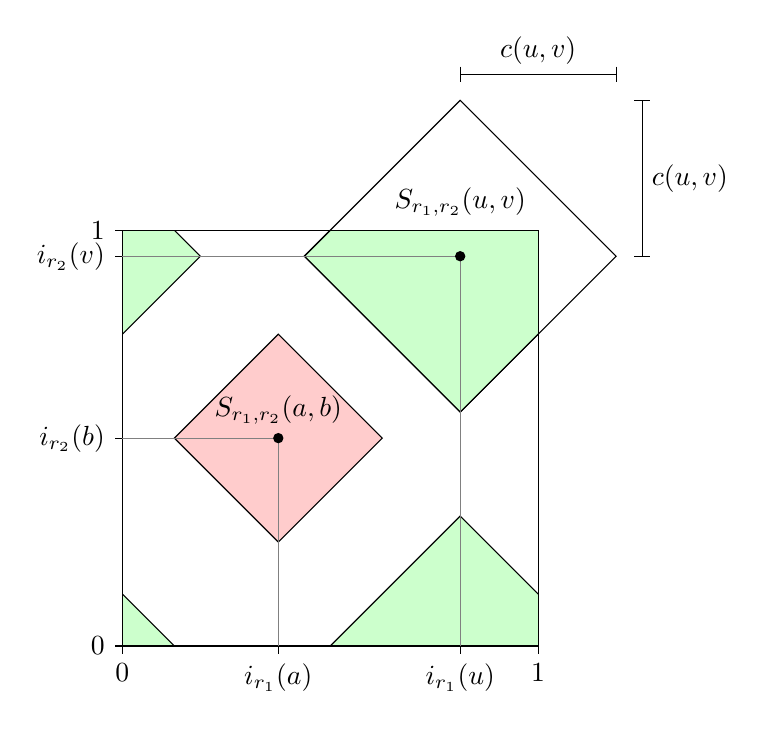
\begin{tikzpicture}[scale=0.33]
\def\firstrect{(13,9) -- (7, 15) -- (13, 21) -- (19, 15) -- (13,9)}
\def\secondrect{(6,4) -- (2, 8) -- (6, 12) -- (10, 8) -- (6,4)}
\begin{scope}
\clip[draw] (0,0) rectangle (16,16);
\begin{scope}[shift={(  0,  0)}] \filldraw[fill=green!20] \firstrect; \end{scope}
\begin{scope}[shift={(-16,  0)}] \filldraw[fill=green!20] \firstrect; \end{scope}
\begin{scope}[shift={(-16,-16)}] \filldraw[fill=green!20] \firstrect; \end{scope}
\begin{scope}[shift={(  0,-16)}] \filldraw[fill=green!20] \firstrect; \end{scope}
\end{scope}
\draw \firstrect;
\filldraw[fill=red!20] \secondrect; 
\draw (0,0) rectangle (16,16);
\draw (0,0) -- (0,-0.3) node[below] {$0$};
\draw (0,0) -- (-0.3,0) node[left]  {$0$};
\draw (16,0) -- (16,-0.3) node[below] {$1$};
\draw (0,16) -- (-0.3,16) node[left]  {$1$};

\draw (13,0) -- (13,-0.3) node[below] {$i_{r_1}(u)$};
\draw ( 6,0) -- ( 6,-0.3) node[below] {$i_{r_1}(a)$};
\draw (0,15) -- (-0.3,15) node[left] {$i_{r_2}(v)$};
\draw (0, 8) -- (-0.3, 8) node[left] {$i_{r_2}(b)$};

\draw[gray] (13,0) -- (13,15) -- (0,15);
\draw[gray] ( 6,0) -- ( 6, 8) -- (0, 8);

\fill (6,8) circle (0.2);
\fill (13,15) circle (0.2);
\draw ( 6, 10) node[below] {$S_{r_1,r_2}(a,b)$};
\draw (13, 18) node[below] {$S_{r_1,r_2}(u,v)$};

\draw (13, 22) -- (19, 22) node[midway, above] {$c(u,v)$};
\draw (13, 22.3) -- (13, 21.7);
\draw (19, 22.3) -- (19, 21.7);


\draw (20, 21) -- (20, 15) node[midway, right] {$c(u,v)$};
\draw (19.7, 21) -- (20.3, 21);
\draw (19.7, 15) -- (20.3, 15);

\end{tikzpicture}
\caption{The sets $S_{r_1,r_2}(a,b)$ (red) and $S_{r_1,r_2}(u,v)$ (green) assigned to the edges $(a,b)$ and $(u,v)$ of a 2-optimal tour. The sets are taken modulo the unit square and thus may consist of up to four parts.}
\label{fig:upperbound}
\end{figure}
\end{frame}


\begin{frame}{}
    \begin{theorem}
The approximation ratio of the 2-Opt on metric TSP is at least
$\sqrt{\frac{n}{2}}$.
\end{theorem}
\pause
Let $G$ be a complete graph on $n := 2\cdot k^2$ nodes with vertex set 
$V(G) := \{v_{i,j} \mid 1\le i,j \le k\} \cup \{w_{i,j} \mid 1\le i,j \le k\}$.
For each $i$ with $1\le i\le k$, we call $V_i := \{ v_{i,j} \mid 1\le j \le k \}$
and $W_i := \{ w_{i,j} \mid 1 \le j \le k \}$ a \emph{section} of $V(G)$
and the $v$-vertices and $w$-vertices the two \emph{halves} of $V(G)$.

We define a distance function $c:E(G)\to\mathbb{R}_{\ge 0}$ as follows:
\begin{align*}
c(v_{i,j}, w_{i',j'}) & =  ~~1  & \mbox{ for all } 1 \le i, i', j, j' \le k \\
c(v_{i,j}, v_{i',j'}) & = 
  \begin{cases}
  0 & i = i' \\
  2 & i \neq i'
  \end{cases} & \mbox{ for all } 1 \le j, j' \le k \\
c(w_{i,j}, w_{i',j'}) & = 
  \begin{cases}
  0 & i = i' \\
  2 & i \neq i'
  \end{cases} & \mbox{ for all } 1 \le j, j' \le k 
\end{align*}

\end{frame}

\begin{frame}{}
    
    \begin{figure}[h]

  \centering\scriptsize
  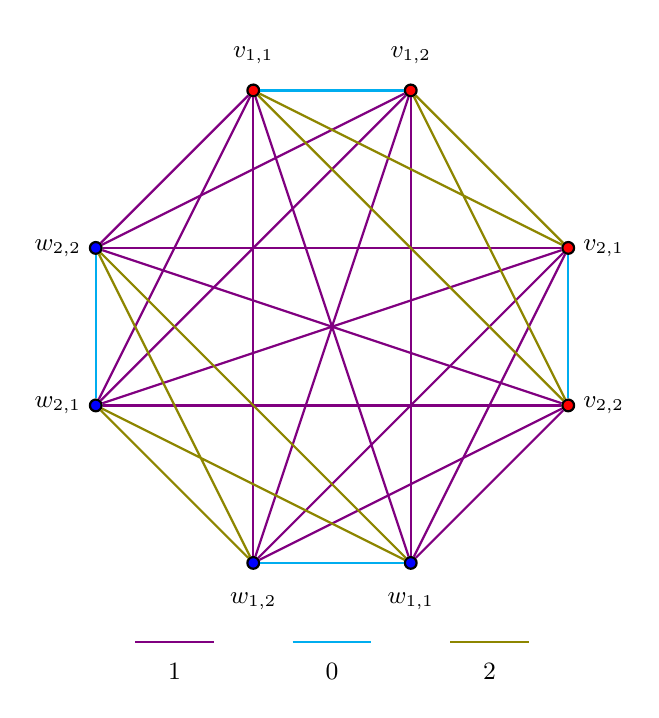
\begin{tikzpicture}[auto=left,every node/.style={circle,draw,inner sep=1.5pt}, every path/.style={thick},scale=.5]
  \node[fill=red,label=above:{\small $v_{1,1}$}] (1) at (4,16) {};
  \node[fill=red,label=above:{\small $v_{1,2}$}] (2) at (8,16) {};
  \node[fill=red,label=right:{\small $v_{2,1}$}] (3) at (12,12) {};
  \node[fill=red,label=right:{\small $v_{2,2}$}] (4) at (12,8) {};
  
  \node[fill=blue,label=below:{\small $w_{1,1}$}] (5) at (8,4) {};
  \node[fill=blue,label=below:{\small $w_{1,2}$}] (6) at (4,4) {};
  \node[fill=blue,label=left:{\small $w_{2,1}$}] (7) at (0,8) {};
  \node[fill=blue,label=left:{\small $w_{2,2}$}] (8) at (0,12) {};
  
  \pause
  \foreach \i in {1,2,3,4} 
     \foreach \j in {5,6,7,8} {
        \draw[violet] (\i) -- (\j) ;
     }
    \draw[violet] (0+1,2) -- (2+1,2);
    \draw (2,0.8) coordinate [label=above:{\small $1$}]();
    
    \pause
    
   \foreach \i\j in {1/2,3/4,5/6,7/8} {
      \draw[cyan] (\i) -- (\j);
   }
    \draw[cyan] (1+4,2) -- (1+6,2);
    \draw (6,0.8) coordinate [label=above:{\small $0$}]();
    \draw[olive] (1+10,2) -- (1+8,2);
    
    \pause
    \draw[olive] (4) -- (1) -- (3) -- (2) -- (4);
    \draw[olive] (7) -- (5) -- (8) -- (6) -- (7);
    \draw (10,0.8) coordinate [label=above:{\small $2$}]();

  \end{tikzpicture}
\end{figure}

    
\end{frame}

\begin{frame}{}
    \begin{align*}
E(T) =~ & \{(v_{i,j}, v_{i,j+1}) \mid 1 \le i \le k, 1 \le j < k \} ~\cup \\
        & \{(w_{i,j}, w_{i,j+1}) \mid 1 \le i \le k, 1 \le j < k \} ~\cup \\
        & \{(v_{i,k}, w_{i,1})   \mid 1 \le i \le k \} ~\cup \\
        & \{(w_{i,k}, v_{i+1,1}) \mid 1 \le i < k \} ~\cup \\
        & \{(w_{k,k}, v_{1,1})\}
\end{align*}

\begin{align*}
E(T') =~ & \{(v_{i,j}, w_{j,i})   \mid 1\le i, j \le k \} ~\cup \\
         & \{(w_{j,i}, v_{i,j+1}) \mid 1\le i \le k, 1 \le j < k\} ~\cup \\
         & \{(w_{k,i}, v_{i+1,1}) \mid 1 \le i < k \} ~\cup \\
         & \{(w_{k,k}, v_{1,1})\}
\end{align*}
\end{frame}

\begin{frame}{}
    \begin{figure}
\centering

\hspace*{-12mm}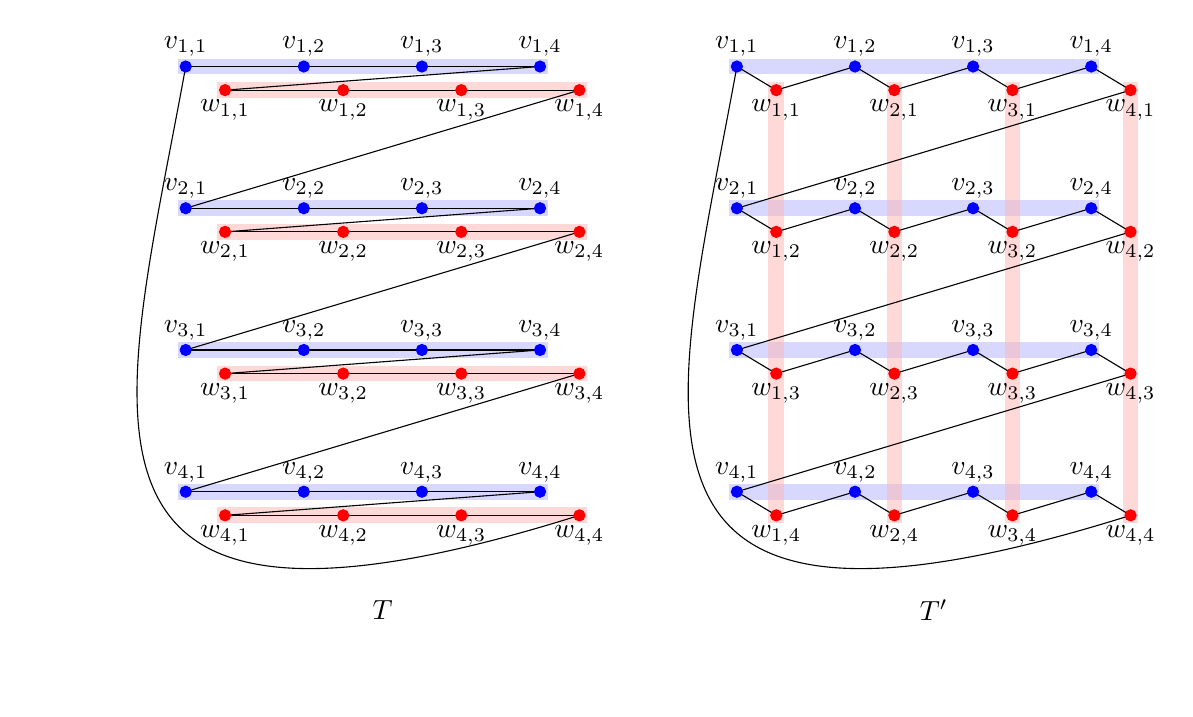
\begin{tikzpicture}
\tikzstyle{vertex_v}=[blue,circle,fill,draw, minimum size=4, outer sep = -0.7mm, inner sep=0]
\tikzstyle{vertex_w}=[ red,circle,fill,draw, minimum size=4, outer sep = -0.7mm, inner sep=0]
\def\yscale{1.8}
\begin{scope}[shift={(0,0)}]
\foreach \y in {0,1,2,3}
    {\fill[blue!30,opacity=0.5] (0-0.1,\yscale*\y - 0.1) rectangle (3 * 1.5 + 0.1,\yscale*\y + 0.1);
     \fill[red!30 ,opacity=0.5] (0-0.1 + 0.5,\yscale*\y - 0.1 - 0.3) rectangle (3 * 1.5 + 0.1 + 0.5,\yscale*\y + 0.1 - 0.3);}


\foreach \x in {0,1,2}
    \foreach \y in {0,1,2,3} 
        {\draw[] (1.5*\x,  \yscale*\y) -- (1.5*\x + 1.5,  \yscale*\y);
         \draw[] (0.5 + 1.5*\x,  -0.3 + \yscale*\y) -- (0.5 + 1.5*\x + 1.5,  -0.3 + \yscale*\y);}
         
\foreach \y in {0,1,2,3} 
    \draw[] (1.5*3,  \yscale*\y) -- (0.5 + 1.5*0,  -0.3 + \yscale*\y);

\foreach \y in {1,2,3} 
    \draw[] (0.5 + 1.5*3,  -0.3 + \yscale*\y) -- (1.5*0,  \yscale*\y - \yscale);
    
\draw[] (0.5 + 1.5 * 3, -0.3 + \yscale * 0) .. controls (-2, -2.5)  and (-0.8, 1) .. (1.5 * 0, \yscale * 3);
         
\foreach \x in {1,2,3,4}
	\foreach \y in {1,2,3,4}
        {\node[vertex_v, label=above:$v_{\y,\x}$] (v\x,\y) at (1.5*\x - 1.5,        4 * \yscale - \yscale*\y) {};
         \node[vertex_w, label=below:$w_{\y,\x}$] (w\y,\x) at (1.5*\x - 1.0, -0.3 + 4 * \yscale - \yscale*\y) {};}
         
\draw (2.5,-1.5) node {$T$};         
\end{scope}

\begin{scope}[shift={(7,0)}]
\foreach \y in {0,1,2,3}
    \fill[blue!30,opacity=0.5] (0-0.1,\yscale*\y - 0.1) rectangle (3 * 1.5 + 0.1,\yscale*\y + 0.1);

\foreach \x in {0,1,2,3}
    \fill[red!30 ,opacity=0.5] (0-0.1 + 1.5*\x + 0.5, - 0.1 - 0.3) rectangle (\x * 1.5 + 0.1 + 0.5, 3*\yscale + 0.1 - 0.3);

\foreach \x in {0,1,2,3}
    \foreach \y in {0,1,2,3} 
        \draw[] (1.5*\x,  \yscale*\y) -- (0.5 + 1.5*\x,  -0.3 + \yscale*\y);

\foreach \x in {0,1,2}
    \foreach \y in {0,1,2,3} 
        \draw[] (1.5*\x + 1.5,  \yscale*\y) -- (0.5 + 1.5*\x,  -0.3 + \yscale*\y);

\foreach \y in {1,2,3} 
    \draw[] (0.5 + 1.5*3,  -0.3 + \yscale*\y) -- (1.5*0,  \yscale*\y - \yscale);
    
\draw[] (0.5 + 1.5 * 3, -0.3 + \yscale * 0) .. controls (-2, -2.5)  and (-0.8, 1) .. (1.5 * 0, \yscale * 3);
         
\foreach \x in {1,2,3,4}
	\foreach \y in {1,2,3,4}
        {\node[vertex_v, label=above:$v_{\y,\x}$] (v\x,\y) at (1.5*\x - 1.5,        4 * \yscale - \yscale * \y) {};
         \node[vertex_w, label=below:$w_{\x,\y}$] (w\x,\y) at (1.5*\x - 1.0, -0.3 + 4 * \yscale - \yscale * \y) {};}

\draw (2.5,-1.5) node {$T'$};         
\end{scope}        
\end{tikzpicture}\\[-1cm]

%\caption{The optimal tour $T$ (left) and the 2-optimal tour $T'$ (right) %for $k = 4$.
%Note that the $w$-vertices on the right are mirrored at the diagonal %compared
%to the $w$-vertices on the left. Thus, on the left, vertices within the %sections $V_i$ and $W_i$ are in a row. On the right, the vertices in 
%the sections $V_i$ are in a row while the vertices in a section $W_i$ are %within a column. 
%The colored bars contain the vertices belonging to the same section.}

\label{metric-picture}
\end{figure}
\end{frame}
\end{document}